\documentclass{article}
\usepackage[utf8]{inputenc}
\usepackage[T1]{fontenc}
\usepackage{tikz}
\usepackage{amssymb} % Necessário para o símbolo \square

% Bibliotecas do TikZ para o diagrama
\usetikzlibrary{automata, positioning, arrows}

% Definindo o comando para o símbolo de branco
\newcommand{\blank}{\square}

\begin{document}

% ==========================================
% PARTE 1: VISUALIZAÇÃO DA FITA (Exemplo)
% ==========================================
\begin{center}
\textbf{Exemplo de Execução (Fita Inicial)}
\vspace{0.5cm}

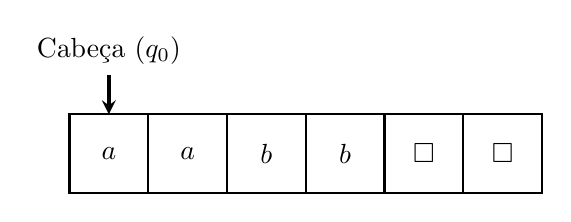
\begin{tikzpicture}[thick]
  % Desenhando a fita: a, a, b, b, branco, branco
  \foreach \sym [count=\i] in {a, a, b, b, \blank, \blank} {
    \draw (\i-1, 0) rectangle +(1, 1);
    \node at (\i-0.5, 0.5) {$\sym$};
  }
  
  % Desenhando a "cabeça" de leitura na posição 1 (q0 lendo 'a')
  \draw[->, >=stealth, very thick] (0.5, 1.5) -- (0.5, 1.0);
  \node[above] at (0.5, 1.5) {Cabeça ($q_0$)};
\end{tikzpicture}
\end{center}

\vspace{1cm}
\hrule
\vspace{1cm}

% ==========================================
% PARTE 2: DIAGRAMA DE ESTADOS (Lógica)
% ==========================================
\begin{center}
\textbf{Diagrama de Estados}
\vspace{0.5cm}

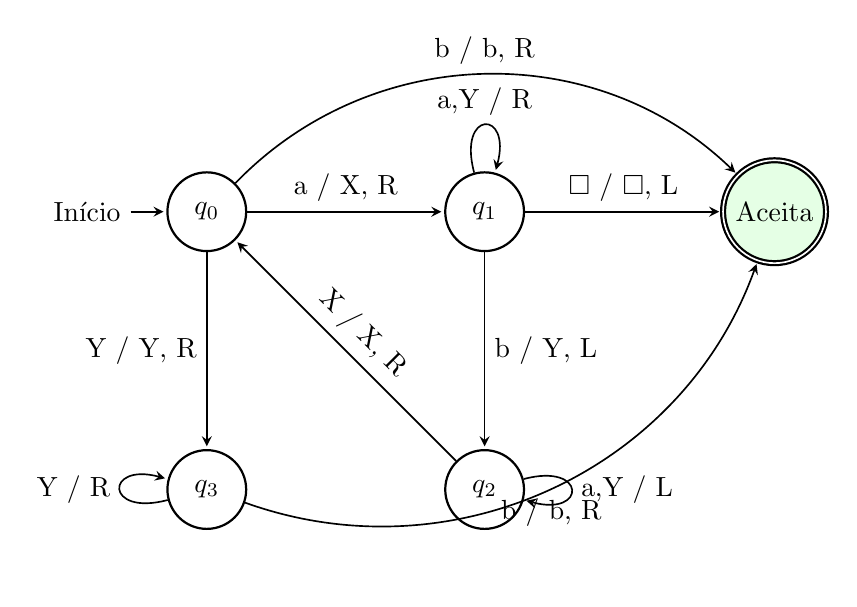
\begin{tikzpicture}[
    ->,                 % Ponta de seta em todas as linhas
    >=stealth,          % Estilo da seta
    shorten >=1pt,      % Espaço pequeno antes de tocar o nó
    auto,               % Posiciona o texto automaticamente
    node distance=2.5cm, % Distância padrão
    semithick,          % Grossura da linha
    state/.style={circle, draw, minimum size=10mm, thick, fill=white},
    accept/.style={double, circle, draw, minimum size=10mm, thick, fill=green!10}
  ]

  % --- DEFINIÇÃO DOS ESTADOS ---
  \node[state, initial, initial text=Início] (q0) {$q_0$};
  \node[state, right=of q0] (q1) {$q_1$};
  \node[state, below=of q0] (q3) {$q_3$};
  \node[state, below=of q1] (q2) {$q_2$};
  \node[accept, right=of q1] (acc) {Aceita};

  % --- TRANSIÇÕES ---
  
  % Do q0
  \path (q0) edge node {a / X, R} (q1)
             edge[bend left=45] node {b / b, R} (acc)
             edge node[left] {Y / Y, R} (q3);

  % Do q1
  \path (q1) edge[loop above] node {a,Y / R} (q1)
             edge node {$\blank$ / $\blank$, L} (acc)
             edge node[right] {b / Y, L} (q2);

  % Do q2
  \path (q2) edge[loop right] node {a,Y / L} (q2)
             edge node[above, sloped] {X / X, R} (q0);

  % Do q3
  \path (q3) edge[loop left] node {Y / R} (q3)
             edge[bend right=45] node[below] {b / b, R} (acc);

\end{tikzpicture}
\end{center}

\end{document}